%
% fig-komplexer-summand.tex
%
% (c) 2026 Prof Dr Andreas Müller
%
\begin{figure}
\centering
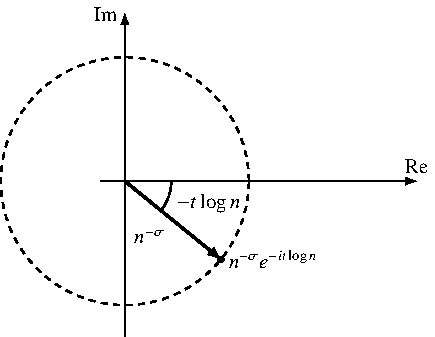
\includegraphics{papers/hankel/images/komplexer-summand.pdf}
%\begin{tikzpicture}[scale=1.05,>=latex]
%	\draw[->] (-0.4,0) -- (4.7,0) node[right] {$\operatorname{Re}$};
%	\draw[->] (0,-2.5) -- (0,2.7) node[above] {$\operatorname{Im}$};
%	\draw[dashed] (0,0) circle[radius=2.0];
%	\draw[->,very thick] (0,0) -- (1.55,-1.26)
%		node[midway,below left] {$n^{-\sigma}$};
%	\draw (0.75,0) arc[start angle=0,end angle=-39,radius=0.75];
%	\node at (1.35,-0.36) {$-t\log n$};
%	\fill (1.55,-1.26) circle[radius=1.5pt];
%	\node[right] at (1.55,-1.26)
%		{$n^{-\sigma}e^{-it\log n}$};
%\end{tikzpicture}
\caption{Betrag und Phase eines Summanden $n^{-s}$ mit $s=\sigma + it$. 
Die Darstellung ist schematisch; der Kreis hat den Radius $n^{-\sigma}$.}
\label{hankel:fig:komplexer-summand}
\end{figure}
